\section{Реализация}
\label{sec:implementation}

В этом разделе наше внимание сместится на особенности реализации процессов
связанных с проверкой типов в Scala Plugin и особенности их инструментирования.
Так как конечной целью является визуализация работы этих процессов, то
хочется максимально опираться на стандарт языка, которым является спецификация
scala \cite{scala_spec}.
Мы проследим как понятия из спецификации переносятся в Scala Plugin.
А там где это не возможно будет явно указано на расхождение в реализации плагина и
спецификации.
Так-же для каждого процесса будет приведен пример его визуализации.

% Реализация в плагине в плагине
% Смысл в последующей визуализации
% Хочется сделать С уважением к спецификации
% Однако не везде это возможно сделать
% Где можно сделаем
% Везде будет указано расхождение

До этого момента, когда мы говорили о работе плагина, то использовали
нейтральное слово процесс.
Теперь нужно вспомнить, что изначальной задачей было явно визуализировать
работу связанную с типами, которую плагин делает неявно.
Архитектура части плагина связанной с типами будет
рассмотрена в разделе \ref{sec:arch}.
Перечислим интересующие нас процессы.

Базовым процессом является сравнение двух типов.
В спецификации для этого вводятся три понятия: эквивалентность типов, сводимость
типов и слабая сводимость типов.
Эквивалентность означает что один тип мы в любом контексте можем заменить другим
типом, и это отношение наиболее понятно интуитивно.
Сводимость типов намного более интересна и используется во всех других процессах.
Ее мы рассмотрим в разделе~\ref{sec:conformance}.
Там же будет описание слабой сводимости, а также будет разобрано представление
типов в Scala Plugin и их отличия от типов описанных в спецификации.

Следующим интересующим нас процессом будет вывод типов.
Важно что вывод типов в плагине и в спецификации осуществляется по разному.
Подробно об этом будет написано в разделе~\ref{sec:infer}

Последний процесс, следующий из вывода типов - это разрешение перегрузок функций.
Действительно, типовые переменные появляются в вызовах полиморфных
функций и их неявный вывод актуален для конкретного вызова.
А так как в scala присутствуют перегрузки функций, то прежде всего нужно
разрешить символ на котором были вызваны аргументы.
Процесс разрешения перегрузок будет рассмотрен в разделе~\ref{sec:overloading}.

Отдельного упоминания заслуживает механизм implicit.
В данной работе не затрагивались неявные преобразования и неявные параметры.
В рамках Scala Plugin уже существуют \textbf{ShowImplicitParametersAction},
показывающий неявно передаваемые параметры и рассмотренный в
разделе~\ref{sec:showImplicit}, и \textbf{GoToImplicitConversationAction},
помогающий в работе с неявными преобразованиями.
Так же в данной работе не освященна работа с динамическими типами.
В будущем эти пробелы можно восполнить.
% \textbf{Еще не уделялось внимания наследованию.}

\subsection{Архитектура Scala Plugin}
\label{sec:arch}

\begin{figure}[t]
\centering
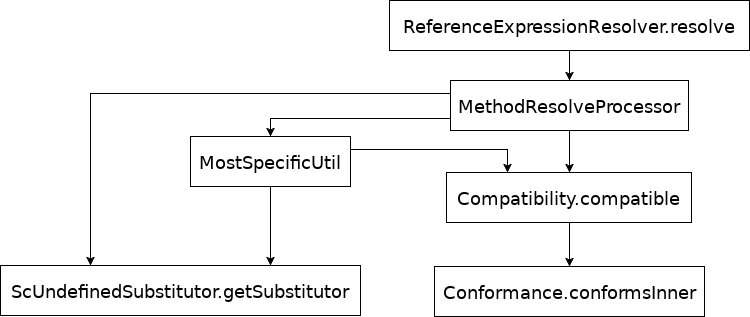
\includegraphics[width=\textwidth]{img/call-graph}
\caption{Граф вызовов}
\label{fig:callGraph}
\end{figure}

Как говорилось в начале раздела~\ref{sec:implementation}, нас будут интересовать
процессы сведения типов, выведения типов и выбора перегрузки функции.
Все эти процессы можно проилюстрировать на вызове полиморфной функции.
Для начала рассмотрим как он будет обрабатываться плагином.
На рисунке~\ref{fig:callGraph}, несколько упрощенно, показан граф вызовов
такой обработки.
Мы явно будем указывать классы, основные и вспомогательные функции в которых
использовалась аннотация \textbf{uninstrumented} из раздела~\ref{sec:features}.
Это поможет дучше понять куда именно добавлялась инструментация.
% основываясь на интересующих нас процессах

% \textbf{Улучшить введение.}
Представим что у нас есть применение символа к набору выражений-аргументов.
Для обработки этого применения у объекта \textbf{ReferenceExpressionResolver}
будет вызван метод \textbf{resolve}.
Это и будет точкой входа.
Аннотировано \textbf{uninstrumented}:
\begin{itemize}
  \item \textbf{ReferenceExpressionResolver.resolve}
\end{itemize}
% Здесь только к методу \textbf{resolve} будет добавлена аннотация uninstrumented.

Далее с помощью класса \textbf{MethodResolveProcessor} будет осуществлен
поиск кандидатов обладающих таким же именем как \textbf{f}.
\textbf{MethodResolveProcessor} будет хранить множество кандидатов и
результаты применения соответсвующих кандидатов к аргументам.
Также там находится часть логики по фильтрации кандидатов, более подробно о которой
будет написано в разделе~\ref{sec:overloading}.
Аннотировано \textbf{uninstrumented}:
\begin{itemize}
  \item \textbf{MethodResolveProcessor}
  % класс
  \item \textbf{MethodResolveProcessor.problemsFor}
  \item \textbf{MethodResolveProcessor.candidates}
\end{itemize}
% Аннотация uninstrumented была добавлена к самому классу
% \textbf{MethodResolveProcessor}, а также к вспомогательным методам
% объекта-компаньона \textbf{problemsFor} и \textbf{candidates}.

Для каждого кандидата нужно проверить, возможно ли вызвать его с такими аргументами.
Инструменты для этого находятся в классе \textbf{Compatibility}.
Омновная часть кода здесь - это перебор разных конструкций Scala Plugin,
описывающих исходный код, а также способов применения к ним аргументов.
Например, разбор таких случаев как: передача аргумента по имени или параметры со
значением по умолчанию.
Аннотировано \textbf{uninstrumented}:
\begin{itemize}
  \item \textbf{Compatibility.checkConformance}
  \item \textbf{Compatibility.checkConformanceExt}
  \item \textbf{Compatibility.compatible}
\end{itemize}
% Здесь аннотация uninstrumented добавлена к методам объекта
% \textbf{checkConformance}, \textbf{checkConformanceExt} и \textbf{compatible}.

Для проверки сводимости двух типов используется интерфейс \textbf{Conformance}.
У этого интерфейса две реализации: одна для системы типов scala, другая для
системы типов dotty \cite{dotty}, нового поколения языка scala.
В обоих случаях метод \textbf{conformsInner} возвращает пару: возможна ли
сходимость и набор ограничений на абстрактные типы при которых сходимость
возможна.
Про процесс проверки сводимости написано в разделе~\ref{sec:conformance}.
Аннотировано \textbf{uninstrumented}:
\begin{itemize}
  \item \textbf{Conformance.conformsInner}
  \item \textbf{Conformance.computable}
  \item \textbf{Conformance.checkParameterizedTypes}
  \item \textbf{Conformance.addParam}
  \item \textbf{Conformance.addArgedBound}
  \item \textbf{Conformance.LeftConformanceVisitor}
\end{itemize}
% Здесь аннотации uninstrumented применяются к методам
% \textbf{conformsInner}, \textbf{computable}, \textbf{checkParameterizedTypes},
% \textbf{addParam}, \textbf{addArgedBound}, а также к
% классу \textbf{LeftConformanceVisitor}.

Далее необходимо проверить что ограничения, полученные на предыдущем шаге,
возможно разрешить.
Для этого есть интерфейс \textbf{ScUndefinedSubstitutor}.
Его реализуют \textbf{ScUndefinedSubstitutorImpl} и
\textbf{ScMultiUndefinedSubstitutor}.
Отличие одной реализации от другой состоит в том, что
\textbf{ScUndefinedSubstitutorImpl} хранит только один набор ограничений, в
то время как \textbf{ScMultiUndefinedSubstitutor} хранит сразу несколько.
Это может понадобится если существует более одного способа добиться сводимости
типов. Конкретно это используется для \textit{compound type}.
Заметим, что разрешение ограничений на абстрактные типы - это и есть вывод типов.
Больше информации можно получить в разделе~\ref{sec:infer} о выводе типов.
Аннотировано \textbf{uninstrumented}:
\begin{itemize}
  \item \textbf{ScUndefinedSubstitutor.addLower}
  \item \textbf{ScUndefinedSubstitutor.addUpper}
  \item \textbf{ScUndefinedSubstitutor.getSubstitutorWithBounds}
  \item \textbf{ScUndefinedSubstitutor.getSubstitutor}
\end{itemize}
% Аннотация uninstrumented используется методах \textbf{addLower},
% \textbf{addUpper}, \textbf{getSubstitutorWithBounds}, а также \textbf{getSubstitutor}.

Интересно заметить, что пара \textbf{Compatibility} и
\textbf{ScUndefinedSubstitutor} образуют что-то вроде алгоритма
Хиндли-Милнера \cite{hindley–milner}.

Остался класс \textbf{MostSpecificUtil}.
Он нужен если после всех проверок сделанных \textbf{MethodResolveProcessor}
осталось больше одного кандитата.
В таком случае требуется найти наиболее специфичного кандитата.
Именно этим \textbf{MostSpecificUtil} и занимается.
Подробнее в разделе~\ref{sec:overloading}.
Аннотировано \textbf{uninstrumented}:
\begin{itemize}
  \item \textbf{MostSpecificUtil}.
\end{itemize}
% С помощью uninstrumented аннотируется только сам класс
% \textbf{MostSpecificUtil}.

% Все это было инструментровано для сбора дополнительных данных.
Всего в проекте потребовалось использовать 28 аннотаций \textbf{uninstrumented}.
Стоит заметить что граф вызовов сильно упрощен для улучшения понимания.
На самом деле по разным причинам все вызывают почти всех.

% Повсюду куча сравнений...\textbf{MethodResolveProcessor} \textbf{Compatibility}


\subsection{Проверка сводимости типов}
\label{sec:conformance}

В этом разделе будет рассмотрен процесс сводимости типов, будут описаны
структуры отвечающие за типы в Scala Plugin, а также дано сравнение типов
используемых Scala Plugin и типов описанных в спецификации scala.

В спецификации scala сводимость ($<:$) вводится как транзитивное замыкание над
набором аксиом и правил вывода.
Это достаточно формальное определение.
Если следовать ему, то любое сведенение типов является некоторым доказательством.
А чтобы убедить кого-то в этом сведении, нужно предоставить корректное дерево
вывода.
Так что алгоритм, который занимается проверкой сводимости двух типов - это
в некотором роде система автоматического доказательства.
Существет множество систем автоматического доказательства \cite{automata},
однако наша логика слишком проста чтобы использовать, например, coq.
Так же стоит отметить, что слабая сводимость - это просто расширение набора
правил вывода для типов наследующихся от \textit{AnyVal}.

В Scala Plugin для проверки сводимости на вход подаются два типа,
далее мы будем называть их левым и правым, задача свести правый к левому.
Для этого у левого типа запускается шаблон посетитель, во время которого
тип конкретизируется, а после происходят проверки основанные на правилах
вывода.
Во время этих проверок посетитель может запускаться еще и для правого типа.
В самом конце идет проверка, является ли правый тип наследником левого.
Подробнее это можно посмотреть в объекте \textbf{Conformance}.

Стоит отметить что, с одной стороны такой подход достаточно прост для анализа.
Однако с другой стороны в нем много избыточности, например, постоянные повторения
одной и той логики для правого и левого типов.
Так же присутствуют постоянные проверки типов на \textbf{Any} и \textbf{Nothing}.
В первый раз они встречаются на самом верхнем уровне, а после проверки
присутствуют в самых неожиданных местах.
В коде можно встретить \textbf{java.lang.Object}, хотя упоминания о
нем в системе типов scala кажется странным.
Забегая вперед, одним из типов в Scala Plugin является \textbf{JavaArray},
который должен быть параметризованным \textbf{scala.Array}.
Отдельная сущность для массива влечет дублирование кода для параметризованных
типов, в котором и так очень много повторений.
Также другия несоответсвия в типах.
Все это сильно повышает неоднородность кода.

\subsubsection{Визуализация}

Теперь поговорим про визуализацию сводимости типов.
Как говорилось в начале главы~\ref{sec:implementation} сведение типов является
базовым процессом, который встречается постоянно и его наглядная визуализация
очень важна.
В качестве способа представления мы будем использовать вложенные вкладки,
которые имеют древовоидную структуру.
Это достаточно естественное решение, учитывая что само сведение является
представляется деревом вывода.

Узлы дерева будут делиться на два типа:
\begin{itemize}
  \item Узлы отношения.
  В этих узлах записано, что рассматриваемые в данный момент
  типы должны состоять в каком-то отношении.
  Это может быть либо правда, либо нет.
  Как пример, можно рассмотреть код~\ref{lst:conformance}.
  В нем мы объявляем отношение сводимости. Оно определено для двух типов:
  правого и левого.
  Для того чтобы оно было истинным, должно быть выполнено хотя бы одно из
  условий сводимости.
  \item Узлы условий.
  Эти узлы символизируют собой аксиомы и правила вывода введенные в спецификации
  scala.
  Часть условий может иметь сложную структуру и требовать выполнения каких-то
  отношений, из-за чего структура получается рекурсивной.
  В коде~\ref{lst:condition} находится интерфейс условия для сводимости.
\end{itemize}


\begin{lstlisting}[caption={Узел условия},label={lst:condition}]
sealed trait CCondition {
  def satisfy(ctx: RelationContext): Boolean
}
\end{lstlisting}

\begin{lstlisting}[caption={Узел отношения},label={lst:conformance}]
case class Conformance(left: ScType, right: ScType,
           conditions: Seq[CCondition]) extends Relation {
  override def satisfy(ctx: RelationContext): Boolean =
    conditions.exists(_.satisfy(ctx))
}
\end{lstlisting}

В обоих случаях во время проверки используется класс \textbf{RelationContext}.
Это нужно чтобы перадть данные полученные во время других процессов.

В ходе работы собираются условия.
После рекурсивных вызовов полученные условия объединяются в отношения.
Мы получаем уже, по сути, готовую для визуализации структуру.
Посмотреть пример результата можно на рисунке~\ref{fig:conformance}.
Далее мы не будем подробно останавливаться на визуализации.
Достаточно знать что она всегда строится примерно одинаково и представляется в
виде дерева.


На этом заканчивается часть про сведение типов в общем и начинается часть про
сводимость для конкретных типов.
Это позволит лучше понять отличия типов представленных внутри Scala Plugin
и спецификацией scala.
Также будет написано как правила вывода из спецификации переносятся в плагин.
Здесь будет дана очень общая информация о типах, чтобы получить более подробную
информацию, например про синтаксис, рекомендуется посмотреть в спецификацию.

% Value Types
%
% Non-Value Types

\subsubsection{Singleton Type}
Scala очень сильно использует концепцию пространств имен.
Причем не только для пакетов или типов.
В scala также у каждой переменной есть свое пространство имен.
За счет этого механизма в scala существует некоторая разновидность зависимых
типов \cite{dependent_types}, а апогеем этой идеи является DOT calculus
\cite{dot_calculus}.

\textit{Singleton type} используется для того чтобы солаться на тип объекта,
пакета или переменной.
Обычно \textit{singleton type} встречается когда мы хотим сослаться на тип объекта.

% правило вывода Singleton продолбано
В плагине этот тип не преставлен классом, а его роль как правило выполняет
\textbf{ScDesignatorType}.
Хоть в спецификации \textit{singleton type} и вводится через концепцию пути,
\textbf{ScDesignatorType} по сути представляет оберку над ссылкой на место в коде,
где соответсвующий объект вводится.
Проверка сводимости для \textit{singleton type}  заменяется на проверку
эквивалентности.
Аксиома о сводимости типа \textbf{Singleton} в плагине отсутвует.

Отдельным случаем в плагине является использование \textit{singleton type} для
ссылки \textbf{this}.
В таком случае нельзя использовать просто ссылку на место в коде.
Нужно учитывать контекст в котором \textbf{this.type} встречается.
Для этого в плагине есть класс \textbf{ThisType} логика обработки которого
сводится к транзитивности и эквивалентности.


\subsubsection{Type Projection}

Любой тип в scala, согласно спецификации, лежит в каком-то пространстве имен.
И сам тип тоже образует пространство имен.
Чтобы получить доступ к типам в пространстве имен типа, используются
\textit{type projection}.
Все классы описываемые пользователем типы, а также стандартные будут такими,
как правило являются \textit{type projection}.
Так, например, тип представляющий целые числа будет выглядеть как
\textbf{scala.type\#Int}.
Здесь мы взяли базовый пакет scala, получли его \textit{singleton type}, а после
спроецировали в \textit{projection type}.

В Scala Plugin есть класс \textbf{ScProjectionType}, который содержит
проецируемый тип и имя проекции.
Для него правила вывода \textit{type projection} добавляются без особых
сложностей.

\subsubsection{Type Designator}
Для того чтобы не писать все время \textbf{scala.type\#Int}, как в предыдущем пукте,
существует \textit{type designator} являющийся коротким синонимом для
\textit{type projection}.
Таким образом \textbf{Int} будет просто сокращением для \textbf{scala.type\#Int}.

Вышеупомянутый \textbf{ScDesignatorType} берет на себя и эту роль.
Правда его связь с \textit{type projections} теряется, остаются проверки
эквивалентности и наследования.
Так же есть тонкость с объявлением абстрактных типов, но про это будет написано
в разделе Abstract Types.

\subsubsection{Parameterized Type}
\textit{Parameterized type} появляется когда у нас есть конструктор типа и мы хотим
применить его к типовым аргументам.
Например, \textbf{List[Int]} - это \textit{parameterized type},
где \textbf{List} - это конструктор типа, принимающий один типовой
аргумент.
Для типовых параметров возможны три вида вариантности:
ковариантность, контрвариантность и инвариантность.
Варинатность влияет на сводимость \textit{parameterized type}.
Ковариантность говорит что параметры должны сводится так же как
\textit{parameterized type}, контрвариантность что наоборот, а инвариантность
что должны совпадать.

В плагине есть соответствующий класс \textbf{ParameterizedType}.
Понятия и правило вывода из спецификации переносятся на него, хоть логика
работы с ним и тяжеловесна.

\subsubsection{Compound Type}
\textit{Compound type} объединяет в себе понятия конъюнктного и структурного
типов.
Идейно, можно представлять что конъюнктный тип \textbf{A with B} является
наибольшим общим предком для типов \textbf{A} и \textbf{B}.
Аналогично для большего количества типов.
С другой стороны существуют структурные типы, определяющиеся набором объявлений
перменных, типов и функций.
Так \textbf{AnyRef \{ def f(): Int \}} - это просто тип у которого есть
метод \textbf{f}, возвращающий \textbf{Int}.
Если какой-то тип доходит под это определение, то он сводится
\textbf{AnyRef \{ def f(): Int \}}.
Если объединить эти две концепции, то получится \textit{compound type}.

В Scala Plugin \textit{compound type} представлен классом \textbf{ScCompoundType}.
Логика работы с ним соответсвуют описанным в спецификации правилам введения и
выведения, которые и требуется добавить.
Интересный момент возникает для ограничений на абстрактные типы.
Например, если мы пытаемся свести тип \textbf{A with B} к типу \textbf{C},
то для этого либо \textbf{A} должен сводиться к \textbf{C}, либо \textbf{B}
должен сводиться к \textbf{C}.
Нас устроит любой из вариантов, однако могут возникнуть разные ограничения на
типы.
Так как ограничения разрешаются в самом конце, то необходимо сохранить все
варианты ограничений.
Именно для этой ситуации и существет класс \textbf{ScMultiUndefinedSubstitutor},
встреченный в разделе~\ref{sec:arch}.

\subsubsection{Existential Type}
\textit{Existential type} - это просто экзестенциальный тип, подробнее о котором
можно почитать в \cite{type_theory}.
Он нужен чтобы замкнуть свободные типовые переменные.
Примером такого типа будет \textbf{List[(A, A)] forSome \{ type A \}}.
Здесь мы объявили список пар, где типы первого и второго элемента пары совпадают.

В Scala Plugin для \textit{existential type} используется класс
\textbf{ScExistentialType}.
Он так же как и \textbf{ParameterizedType} добавляет к типу набор переменных,
только тут эти переменные должны быть абстрактными.
Класс представляющий абстрактную типовую переменную в \textit{existential type}
называется \textbf{ScExistentialArgument}.
В нем содержится информация об имени и границах типа, а также типовых агрументах.
Последнее нужно для поддержки типов высших кайндов.
Правила ввода и вывода можно брать из спецификации.
Интересный момент возникает при сведении какого-нибудь типа к \textit{existential type}.
В таком случае требуется не просто найти ограничения для типовых параметров,
нужно проверить что они разрешимы, а все условия на границы типов соблюдены.
Поэтому тут решение системы ограничений на типы происходит прямо во время сведения.

\subsubsection{Method Type}

Как известно, в scala функции являются объектами первого порядка.
Иначе говоря, мы можем передавать функции как аргументы, сохранять в переменные
и так далее.
Однако, мы не всегда можем выразить различные типы методов, доступные в scala,
через классы с дженериками.
Поэтому для описания методов вводится отдельный тип, называемый \textit{method type}.
Этот тип нельзя выразить в синтаксисе scala, а при необходимости привести
\textit{method type} к типу функции, выполняется эта-расширение~\cite{eta_expansion}.

В плагине используется есть соответсвующий класс \textbf{ScMethodType}.
Так как \textit{method type} можно свести только к \textit{method type}, его
обработка локализована и в точности повторяет то что написано в спецификации.
Поэтому правило сведения можно переносить напрямую.

\subsubsection{Polymorphic Method Type}
Что бы представить в типы зависящие от типов, такие как полиморфные методы,
используется \textit{polymorphic method type}.
Таким образом это он является типом, принимающим типовые аргументы,
и возвращающим некоторый внутрениий тип с подставленными аргументами.
Его так же как и \textit{method type} нельзя выразить синтаксически.

В Scala Plugin его представляет \textbf{ScTypePolymorphicType}, который содержит
внутренний тип и набор типовых параметров.
Работа с ним повторяет правило вывода из спецификации.

\subsubsection{Type Constructors}
Отдельным случаем в спецификации scala рассматриваются типовые конструкторы.
В этом случае применение типовых аргументов приводит к типу который можно
инстанцировать.

В Scala Plugin его роль выполняет все тот же \textbf{ScTypePolymorphicType}.
Поэтому это не добавляет нового правила вывода.

\subsubsection{Abstract Type}

\textit{Abstract type} не вводится среди основных типов в спецификации, однако
упоминается в самом начале соответсвующего раздела.
Он определяется как тип описываемый типовым параметром или объявление типа без
конкретного значения.
При работе с ним используются его верхняя и нижняя границы.

В Scala Plugin под этот случай можно подвести много классов.
В первую очередь это \textbf{TypeParameterType} который используется как тип
типового параметра.
Аналогичные правила применяются для встреченного ранее
\textbf{ScExistentialArgument}.
И сюда же попадает \textbf{ScDesignatorType}.
Как говорилось ранее, он ссылается на куски кода.
При объявления типов без конкрентных значений используется он же.
Для работы со всеми ними можно использовать аксиомы для работы с \textit{abstract type}.

\subsubsection{Типы представленные только в спецификации scala}
Так же в scala спецификации вводятся такие типы как \textit{annotated type} и
\textit{infix type}, но первый не важен в рассматриваемых нами процессах,
а второй является просто синтаксическим сахаром.

Еще есть \textit{tuple type} и \textit{function type}.
Первый является удобной формой записи для кортежа, а второй для функции.
Оба этих типа являются синтаксическим сахаром и сводятся к параметризованным
типам в scala.
Но это не обязательно правда для dotty.
В плагине нет типов соответсвующих им, вместо этого он сразу производит
удаление синтаксического сахара.
Подробнее про это можно прочитать в работе \cite{kozlov}.

\subsubsection{Типы представленные только в Scala Plugin}
Хоть в Scala Plugin и отсутсвуют и отсутсвуют такие сущности как
\textit{tuple type} или \textit{function type}, зато он привносит
свои понятия в систему типов.

Первое о чем хочется сказать - это класс \textbf{JavaArray}.
Он абстрагирует массивы из java.
Правило вывода такое же как у \textit{parameterized type}.
Вместо массивов в scala используется конструктор типа \textbf{scala.Array} и
не совсем понятно, почему сразу не сделать преобразование к соответствующему
параметризованному типу.
Возможно наличие такого класса и удобно в каких то местах, но это никак не
помогает в работе с типами.
Более того, это вызывает дублирование, и без того громоздкой, логики для
параметризованных типов.
Также стоит заметить что как язык, scala постепенно отходит от своей привязки к jvm.
У него постепенно появлются новые платформы, такие как scalajs \cite{scalajs}
или scala native \cite{scala_native}.

\textbf{StdType} это перечислимый тип содержащий в себе такие вещи как
\textbf{Long}, \textbf{Double}, \textbf{Int}...
Самое интересное - это \textbf{Any}, \textbf{AnyRef}, \textbf{Null} и
\textbf{Nothing}, так как для этих типов в спецификации существуют отдельные
правила, которые и были перенесны.

Так же в плагине появляются классы \textbf{ScAbstractType} и \textbf{UndefinedType}.
Эти типы используются во время вывода типов и о них будет рассказано в
разделе~\ref{sec:infer}.

\subsection{Вывод типов}
\label{sec:infer}

Говоря про вывод типов, прежде всего стоит отметить что он является локальным.
Это означает что за один раз тип выводится для конкретного выражения.
Также стоит помнить что для вывода типов в общем случае требуются ожидаемый тип
и выражение в типе которого содержатся типовые переменные.
Тогда мы пытаемся свести тип выражения к ожидаемому типу, в процессе получая
ограничения на типовые переменные.
Разрешая эти ограничения, получаются значения для типовых переменных.
Или ошибка компиляции.

Сначала мы рассмотрим вывод типов описанный в спецификации scala.
Пусть \textit{expr} - это выражение в типе которого присутствуют типовые переменные.
Выделяются три случая:
\begin{itemize}
  \item $\mathit{expr}.x$ - мы выбираем имя $x$ у \textit{expr}.
  Тогда вывод типов будет осуществлен для $\mathit{expr}.x$.
  Это нужно для того чтобы использовать ожидаемое значения или получить
  информацию от использования $x$.
  Например, это позволит написать выражение \textbf{Set.empty + 1} и его тип
  выведется как \textbf{Set[Int]}.
  \item \textit{expr} - используется как значение.
  Тогда нужно найти подстановку типовых параметров которая окажется
  непротеворечивой.
  Как именно искать такую подстановку спецификация умалчивает.
  \item $\mathit{expr}(d_1, ..., d_n)$ - мы применили какие-то подвыражения.
  Тогда в первую очередь нужно типизировать $d_i$.
  В спецификации предлагается два способа:
  либо использовать типовые переменные как типовые константы,
  либо, если первый способ не сработал, заменить типовые переменные на \textit{undefined}.
  Здесь \textit{undefined} - это специальный для которого правила вывода
  $\forall T (T <: \mathit{undefined} \land \mathit{undefined} <: T)$.
  Так или иначе, мы типизируем подвыражения.
  После этого мы можем проверить сводимость их типов к ожидаемым значениям и
  получить дополнительные ограничения на типовые переменные.
\end{itemize}

В любом случае вывод типов начинается с какого-то полиморфного метода в который
мы не добавили типовые параметры явно.

В Scala Plugin вывод типов устроен иначе.
Выше уже говорилость что в процессе сведения мы получаем ограничения необходимые
чтобы сводимость выполняется.
Для этого используется тип \textbf{UndefinedType}.
Он удовлетворяет правилам вывода \textit{undefined} из спецификации, при этом
добавляет соответствующее ограничение на типовую переменную которую представляет.
Однако есть существенное различие.
В спецификации \textit{undefined} появляется вместо типовых переменных
ожидаемого типа, то в нашем случае это типовые переменные выражения.

Важным отличием является отсутсвие отсутсвие стадии замены типовых переменных на
типовые константы. В плагине типовые перменные сразу заменяются на
\textbf{ScAbstractType}.
Этот тип похож, в каком-то смысле, на \textit{undefined}.
\textbf{ScAbstractType} хранит в себе ограничения на соответствующую типовую
переменную, доступные из контекста.
Например, в коде~\ref{lst:abstract} в процессе вывода типа выражения
\textbf{magic}, тип \textbf{T} будет представлен как \textbf{ScAbstractType} и
его нижней границей будет \textbf{Int}.

\begin{lstlisting}[caption={Пример ScAbstractType},label=lst:abstract]{Name}
def id[T](t: T): T = t
def magic[U]: U = throw new Exception("no_magic")
val i: Int = id(magic)
\end{lstlisting}

В процессе сводимости эта дополнительная информация используется для
того чтобы прервать заведому бессмысленную проверку.
Так, если \textbf{ScAbstractType} ограничен сверху классом \textbf{Derived},
а мы пытаемся свести к нему \textbf{Base}, то это не даст разумного результата.
Так же информация о границах вносит существенный вклад для ограничений
получаемых \textbf{UndefinedType}.

Все информация связанная с типовыми переменными собирается с помощью этой пары:
\textbf{UndefinedType} и \textbf{ScAbstractType}.
Для них были добавлены соответсвующие правила вывода.

В случае если проверка сводимости завершилась успешно то \textbf{Conformance}
возвращает \textbf{ScUndefinedSubstitutor} хранящий ограничения для всех типовых
переменных встреченных во время проверки.
% После проверки сводимости всех аргументов
Следующий шаг - проверка разрешимости ограничений на типы.
Она выполнено довольно просто.
Для каждой типовой переменной хранится множества верхних и нижних границ.
Сначала находится наименьший тип лежащий выше всех ограничивающих снизу типов.
После, аналогично, находится наибольший тип лежащий ниже всех ограничивающих
сверху типов.
Проверяется их непротеворечивость.

Инструментация сохраняет данные о границах.
В зависимости от вариантности добавляет значения для типовых перменных не
встреченных в проверках сводимости.
А после добавляет эту информации к проверяемой функции.

Во время визуализации информация про выведенные типы попадает в контекст
\textbf{RelationContext}, который был коде~\ref{lst:condition} и
коде~\ref{lst:conformance}.
Эти данные необходимы для большей наглядности.

Пример можно посмотреть на рисунке~\ref{fig:infer}.

\subsection{Разрешение перегрузок функций}
\label{sec:overloading}

Последним рассматриваемым нами процессом будет выбор перегрузки функции.
Как и впрошлый раз, посмотрим как процесс описывается в спецификации scala,
а уже потом перейдем к реализации в Scala Plugin.

Допустим что существует несколько объявлений имени \textbf{f}.
% тогда пусть множество таких объявлений назывется \textit{A}.
Далее будут описаны несколько стадий, каждая из которых должна отсеять
потенциальных кандидатов по какому-либо признаку.
Если после какой-то стадии остался один кандидат, то он считается правильной
перегрузкой, если ни одного, то это ошибка компиляции.
Если в конце кандидат не один, то это тоже ошибка компиляции.

\begin{enumerate}
  \item В первую очередь вводится понятие \textit{shape} для выражения
  \textit{e} по следующим правилам
  \begin{itemize}
    \item если \textit{e} - функция $\mathit{T \Rightarrow b}$,
    то $\mathit{shape}(\mathit{e})$ это $\mathit{Any \Rightarrow shape}(\mathit{b})$
    \item для именнованного параметра имя сохраняется
    \item во всех остальных случаях \textit{Nothing}
  \end{itemize}

  Заметим, что тип выражения \textit{e} всегда сводится к $\mathit{shape}(\mathit{e})$.
  Тогда оставим только тех кандидатов, которые применимы к аргументам, тип которых
  мы упростили до \textit{shape}.

  Это важная стадия, она позволяет выбрать кандидата не опираясь на конкретные
  типы аргументов.
  Это важно, потому что часто для вывода типа аргумента требуется ожидаемое
  значение, а его не узнать пока мы не выберем кандидата.

  \item Типизируем выражения переданные в качестве аргументов без ожидаемого типа.
  Оставим только тех кандидатов, которые можно применить к этим типам.

  \item Оставим только тех кандидатов, которые не используют параметров по умолчанию.

  \item Иначе нужно выбрать наиболее специфичного кандидата.
  Для определения наиболее специфичного кандадта, нужно найти того, кто более
  специфичен чем все остальные.

  Существет два критерия чтобы понять что один кандидат более специфичен чем
  другой.
  \begin{itemize}
    \item Один кандидат объявлен в пространстве имен унаследованном от другого
    кандидата.
    \item Один кандидат сводится к другому кандидату. Для методов это означает
    что аргументы одного метода всегда применимы к другому.
  \end{itemize}
\end{enumerate}

В Scala Plugin отбор кандидатов происходит в классе
\textbf{MethodResolveProcessor}.
Первые кандидаты уже будут отфильтрованы по \textit{shape}, что хорошо.
Иначе бы показывались все варинаты, даже не подходящие по количеству аргументов.
Однако, при этом могло не учитываться наличие некорректных именованных аргументов.
Реализуется совсем странно.

В первую очередь плагин проверяет применимость кандидатов к переданным в
каестве аргументов выражениям.
Все это происходит с помощью \textbf{Compatibility} и
\textbf{ScUndefinedSubstitutor}, и описывалось ранее.
Инструментация сохраняет данные полученные в результате этих проверок.

Далее идут проверки на неправильные именованные аргументы,
а также аргументы со значениями по умолчанию.
Их результаты тоже сохраняются.

По спецификации scala остается найти наиболее специфичного кандидата.
Это происходит внутри класса \textbf{MostSpecificUtil}.
Происходящее там по большей части повторяет написанное в спецификации.

Результат работы для перегруженных функций продемонстрирован на
рисунке~\ref{fig:overloading}.
